\section{Introduction}

Abstraction of word-level functionality from bit-level descriptions of
digital circuits is an important fundamental problem in Electronic
Design Automation (EDA) and design verification. Word-level abstractions
find applications in high-level/RTL datapath synthesis
\cite{demicheli:iccad_98} \cite{demicheli:dac_99}
\cite{demicheli:tcad_03}, RTL verification \cite{WLS} \cite{arditi:bmd}
\cite{lpsat}, word-level SMT and constraint solving \cite{ms:research}
\cite{boolector} \cite{tew:iccad08}, and can also be
applied to detect malicious modifications to a circuit -- potentially
inserted as hardware Trojan horses -- by reverse-engineering the
function implemented by the circuit. It is further desirable that the
obtained word-level abstraction be a {\it canonical} representation of
the function, to facilitate equivalence verification between a
specification model and an implementation circuit. This master's
thesis proposes the investigation of the problem of deriving word-level,
canonical, polynomial representations from circuits over Galois fields
using concepts from commutative algebra and algebraic geometry ---
notably, Gr\"obner bases \cite{gb_book}, Buchberger's algorithm
\cite{buchberger_thesis}, elimination ideals \cite{ideals:book}, 
and the FGLM algorithm \cite{fglm}. 

The main motivation for this work is to ``reverse engineer'' or
identify the function implemented by a given Galois field arithmetic 
circuit as used in Elliptic Curve Cryptography (ECC). The main
operations of encryption, decryption and authentication in ECC rely on
point-addition and point-doubling operations on elliptic curves
defined over Galois fields $\Fkk$. These primitive operations are, in
turn, implemented as circuits that perform polynomial computations
over $k$-bit vectors \cite{eccld}. 
%Moreover, the datapath size $k$ in these applications
%can be very large, {\it e.g.} $k = 163, 233$ and larger, as specified
%by the US National Institute for Standards and Technology (NIST) for
%ECC. 
The objective is to apply our approach to a given circuit and
{\it extract  the word-level polynomial function} implemented by
it for design verification. The mathematical problems addressed in
this proposal, and the approaches to solve them, are described below:

{\bf Problem Statement:} Given a combinational circuit $C$ with
$k$-bit inputs and $k$-bit outputs, such that the circuit implements 
Boolean functions that are mappings between $k$-dimensional Boolean
spaces: $f: \B^k \rightarrow \B^k$. Let $\{a_0, \dots, a_{k-1}\}$
denote the primary inputs of the circuit, and let $\{y_0, \dots,
y_{k-1}\}$ denote the bit-level primary outputs. Suppose that we do
not know the function implemented by the circuit. We wish to
derive a {\it word-level, symbolic representation} of the function as
$Y = \F(A)$, where $Y = \{y_0, \dots, y_{k-1}\}$, $A = \{a_0, \dots, 
a_{k-1}\}$ are, respectively, the output and input bit-vectors,
and $\F$ denotes a polynomial representation of the
function $f$. We wish to further generalize our approach to any
circuit with arbitrary number  of inputs ($n$) and outputs ($m$), as
polynomial functions $f: {\mathbb{F}}_{2^n} \rightarrow
{\mathbb{F}}_{2^m}$. 

{\bf Approach:} At a Boolean-level, canonical symbolic DAG
representations of functions have been extensively investigated; such
as decisions diagrams (ROBDDs \cite{BRYA86}, FDDs \cite{okfdd}),
moment diagrams (BMDs \cite{bmd}, K*BMDs \cite{kbmd}) and their
word-level variants \cite{WLS}. However, the decomposition principle
behind these representations is based on (variants of) the Shannon's
expansion, which is a bit-wise, Boolean decomposition. Such
approaches cannot be efficiently applied to word-level abstraction of
modulo-arithmetic circuits over Galois extension fields
$\Fkk$. Therefore, we approach this problem from a symbolic commutative
algebra perspective. 


The function $f: \B^k \rightarrow \B^k$ is a
mapping among $2^k$ elements. Therefore, $f$ can also be interpreted,
algebraically, in the following two ways: i) as a function $f:
\Z_{2^k} \rightarrow \Z_{2^k}$, i.e. as a function over finite integer
rings $\pmod{ 2^k}$; and ii) as a function $f: \Fkk \rightarrow \Fkk$,
where $\Fkk$ represents the Galois field of $2^k$
elements. In this work, we will analyze $f$ as a polynomial function
over $\Fkk$, for the following reasons. 

First of all, {\it not every
  function} of the type $f: \Z_{2^k} \rightarrow \Z_{2^k}$, is a
polynomial function; i.e. every function cannot be represented by a
polynomial $\F \pmod{ 2^k}$.  In commutative algebra, identification of
such polynomial functions is an important problem: i.e.  given a function
$f: \Z_n \rightarrow \Z_n$, $n \in {\mathbb{N}}$, identify if $f$ has
a polynomial representation. If so, derive a unique,
minimal, canonical polynomial $\F$, such that $f \equiv  \F \pmod{
  n}$. 
%that represents $f$. 
%This
%requires to analyze $f$ at each of the $n$ points, and to setup a
%system of $n$ linear congruences to solve. If this system of
%congruences has a solution, then $f$ is a polynomial function; 
%otherwise, $f$ is not a polynomial function. And the feasible
%solutions to these linear congruences correspond to the coefficients
%of a polynomial $\F$ that represents $f$.  
The papers
\cite{singmaster} \cite{chen_95} \cite{chen_96} addressed such
problems in number theory and algebra. {\it
 Shekhar} \cite{shekhar:phd} also addressed RTL verification of
polynomial datapaths over $k$-bit vectors using the above
concepts. However, in her work, the RTL datapath was already known to
be a polynomial function $\pmod{ 2^k}$. Unfortunately, an arbitrary
$k$-input/$k$-output combinational circuit cannot always be modeled as
a polynomial function over $\Z_{2^k}$; therefore, the $\Z_{2^k}$ model
is not considered in this work. 

On the other hand, there is a well-known ``textbook'' result
\cite{ff:1997} which states that over Galois fields ($\Fq$) of $q$
elements, {\it every function} $f: \Fq \rightarrow \Fq$ is a
polynomial function. 
%By analyzing $f$ over each of the $q$ points, one can apply
%Langrange's interpolation formula and interpolate a polynomial $\F(x)
%= \sum_{k=1} ^q  \frac{ \prod_{i \neq k}  (x -x_i)}{\prod_{i \neq k}
%  (x_k -x_i)} \cdot f(x_k)$, which is a polynomial of degree at 
%most $q-1$ in $x$. One can easily see that $\F(a)=f(a)$ for all $a \in
%\Fq$, and $\F(x)$ is therefore the polynomial function representation
%of $f$. 
Motivated by this fundamental result, we will devise an approach
to extract a word-level polynomial function (abstraction) from a
circuit. Given the circuit $C$ which represents a function $f:
\B^k \rightarrow \B^k$, we will interpret $f$ as a function $f: \Fkk
\rightarrow \Fkk$, and derive a unique, minimal, canonical polynomial
representation as $Y = \F(A)$ over $\Fkk$, where $Y, A$ are,
respectively, the output and input bit-vectors of the circuit
$C$. 
%Note, however, that we are not given a function (mapping);
%rather, we are given a circuit, which is an encoding of the
%function. Interpolating a polynomial $\F$ over $2^k$ points is
%also going to be infeasible for large values of $k$. Therefore, 
We will extract a set of polynomials (ideal) from the circuit and employ
{\it Gr\"obner bases} techniques to abstract the canonical polynomial
representation. Our approach can be generalized to a circuit with
arbitrary number of inputs and outputs, i.e. to analyze polynomial
functions $f: \Fq^d \rightarrow \Fq$, $q = 2^k$, and further to $f:
{\mathbb{F}}_{2^n} \rightarrow {\mathbb{F}}_{2^m}$. 

\begin{Example}
{\bf Motivating Example:} {\it
Consider a 2-bit multiplier circuit over ${\mathbb{F}}_{2^2}$ given in
Fig. \ref{fig:mul2bit}, which implements a function $f: {\mathbb{F}}_4
\times {\mathbb{F}}_4 \rightarrow {\mathbb{F}}_4$. It implements a
{\bf polynomial function}: $Z = A \times B, ~Z, A, B \in
{\mathbb{F}}_4$. Variables $a_0, a_1, b_0, b_1$ are primary inputs,
$z_0, z_1$ are primary outputs, and $s_0, s_1, s_2, s_3, r_0$ are
intermediate variables of the circuit. 
These bit-level variables are in ${\mathbb{F}}_2 = \{0, 1\}$.
%variables $a_0, a_1, b_0, b_1, g_0, g_1, s_0, s_1, s_2, s_3, r_0$ are
%in ${\mathbb{F}}_{2}$. 
Then, we can consider $A = a_0 + a_1 \alpha, ~B = b_0 +
b_1 \alpha$ as the word-level inputs and $Z = z_0 + z_1 \alpha$ 
as the output in ${\mathbb{F}}_4$. Here $P(x) = x^2 + x + 1$ is the primitive
polynomial of ${\mathbb{F}}_4$ and $P(\alpha) = 0$. 
\begin{figure}[htb]
\centerline{
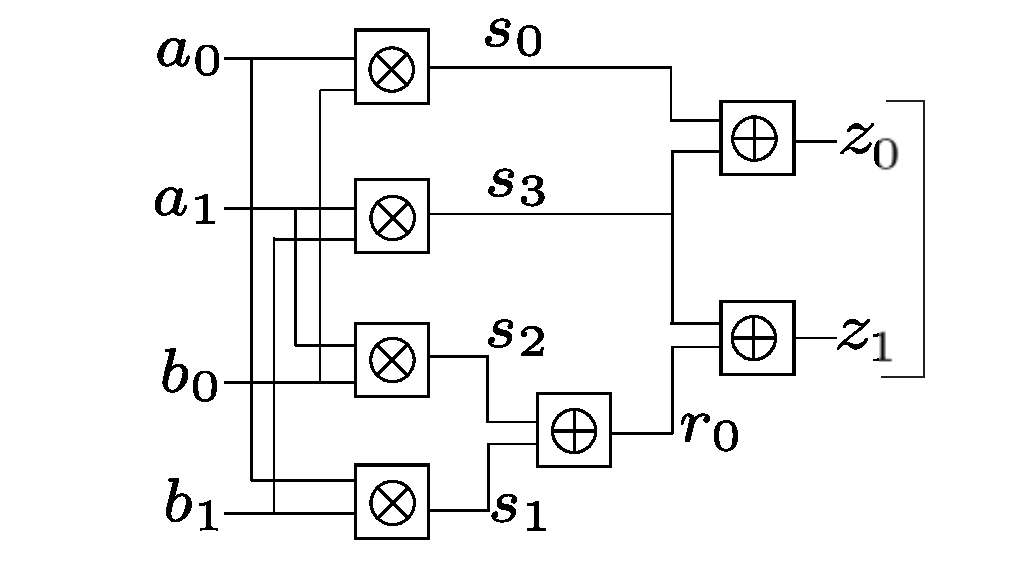
\includegraphics[scale=0.4]{2bitmult.eps}
}
\caption{\small A 2-bit Multiplier over ${\mathbb{F}}_{2^2}$. The gate
  $\otimes$ corresponds to AND-gate, i.e. bit-level multiplication
  modulo 2. The gate $\oplus$ corresponds to XOR-gate, i.e. addition
  modulo 2.} 
\label{fig:mul2bit}
\end{figure}

The functionality of the entire circuit can be described using the
following polynomials derived from the Boolean gate-level operators: 
$f_1: z_0+z_1\alpha +Z; ~~f_2: b_0+b_1\alpha +B; ~~f_3: a_0+a_1 \alpha
+A; ~~f_4: s_0+a_0 \cdot b_0; ~~f_5: s_1+a_0 \cdot b_1; ~~f_6:
s_2+a_1 \cdot b_0; ~~f_7: s_3+a_1 \cdot b_1; ~~f_8: r_0+s_1 + s_2;
~~f_9: z_0+s_0 + s_3; ~~f_{10}: z_1 + r_0 + s_3$. If we impose the
following {\bf elimination} term order: {\bf lex term order} with
``circuit variables'' $>$ ``Output Z'' $>$ ``Inputs, A, B''
%More precisely, we can use {\bf lex} term order with $s_0 > s_1 >  s_2 >
%s_3 >  r_0 > a_0 > a_1 > b_0 > b_1 > g_0 > g_1 > A > B > G$.
%The above term order is an {\bf elimination} order. If we use the above
and compute a Gr\"obner basis $G$ of $\{f_1, \dots, f_{10}\}$, we observe
the following polynomials in the basis:  $g_1: z_0+z_1\alpha +Z;
~~g_2: b_0+b_1\alpha +B; ~~g_3: a_0+a_1 \alpha +A; ~~g_4: s_3+r_0+z_1;
g_5: s_1+s_2+r_0; ~~g_6: s_0+s_3+z_0; ~~{\mathbf{g_7: Z +  AB}}; ~~g_8:
a_1b_1+a_1B+b_1A+z_1; ~~g_9: r_0+a_1b_1+z_1; ~~g_{10}:
s_2+a_1b_0$. Notice that the polynomial $g_7: Z + AB$ describes $Z =
AB$ as the (canonical) polynomial function implemented by the circuit;
and we were able to {\it extract} this representation using the
Gr\"obner basis computation. We wish to explore such an approach to
derive an efficient decision procedure for word-level abstraction. 
}
\end{Example}

%\subsection{Contributions of this Thesis}
{\bf Contributions of this Thesis:} Our approach to solve this
problem, and the contributions of this thesis, can be outlined as
follows: 

\begin{enumerate}
\item Using polynomial abstractions, we analyze the circuit, and
  model the gate-level Boolean operators as elements of a multivariate
  polynomial ring with coefficients in $\Fkk$.

\item Based on the concepts of {\it Strong Nullstellensatz, Gr\"obner
  bases, elimination ideals and projections of varieties}
  \cite{ideals:book}, we deduce that the polynomial abstraction
  problem can be formulated as one of {\it computing a Gr\"obner
    basis} of the set of polynomials derived from the given circuit
  netlist, using a specific elimination term order $>$.

\item Computing Gr\"obner bases using elimination term orders is
  infeasible for large circuits. To overcome this limitation, we will
  investigate the use of the FGLM algorithm \cite{fglm} to derive the
  polynomial representation. The FGLM algorithm takes an {\it already
    computed} Gr\"obner basis ($G_1$) w.r.t. an arbitrary term order
  $>_1$, and transforms it into another Gr\"obner basis ($G$)
  w.r.t. an elimination term order $>$. In the PhD thesis of {\it
  Lv} \cite{lv:phd}, it was shown that for any given
  circuit, there exists a term order $>_1$ that renders the set of
  polynomials derived from the circuit itself a Gr\"obner
  basis. Moreover, $>_1$ can be easily derived by performing a reverse
  topological traversal of the circuit. Consequently, $G_1$ is readily
  available as a Gr\"obner basis directly by construction. Using FGLM,
  we can then translate $G_1$ into the Gr\"obner basis $G$
  w.r.t. the required elimination order $>$. 

\item The worst-case complexity of computing a Gr\"obner basis is
  known to be doubly exponential in $n$, the number of variables, and
  polynomial in $d$, the degree of the ideal. Most hardware/software
  verification applications do exhibit such high complexity, as the
  number of intermediate computations in the Buchbeger's algorithm
  \cite{buchberger_thesis} 
  tend to explode. Therefore, we conjecture that using the FGLM
  algorithm --- which relies on sparse linear algebra concepts ---
  perhaps this complexity can be avoided. In this thesis, we will
  develop a CAD framework using the above ideas and investigate the
  scalability of our methods.

\item As an application, we will use our CAD approach to
  reverse-engineer the function implemented by a given Galois field
  arithmetic circuits used in ECC   implementations. This can be used
  for function identification from a given circuit for formal
  verification. 

\end{enumerate}

{\bf Proposal Organization:} The next section reviews previous work in
the area of canonical representations functions, word-level
abstractions, formal design verification using computer algebra
techniques, and also polynomial interpolation literature in symbolic
computing. Section \ref{sec:prelimgf} reviews 
Galois field theory and hardware design. Section \ref{sec:ideals}
reviews preliminary computer-algebra concepts related to ideals,
varieties, Gr\"obner bases, elimination ideals and
Nullstellensatz. Section \ref{sec:theory} describes our results on
polynomial abstraction from circuits, and demonstrates the application
of our work using preliminary experiments. The application of the FGLM
algorithm is covered in Section \ref{sec:fglm}. Finally, Section
\ref{sec:obj} outlines the research plan and concludes the proposal. 
